\chapter{Sistema Multiagentes}

\section{Teoria dos Grafos}
No estudo da interação e comportamento entre sistemas dinâmicos, as interconexões entre os agentes e o fluxo de informações formam uma rede de comunicação. Essa rede é modelada através da teoria dos grafos em que cada sistema é representado por um nó, também chamado de agente.
% Adicionar Referência do livro que fala sobre

Um grafo é um par $G = (V, E)$, tal que $V = \{v_{1},v_{2}, ...,v_{N}\}$ é um conjunto de $N$ nós ou vértices e $E$ um conjunto de vetores ou arcos. Um elemento pertencente a $E$ é um par $(v_{i}, v_{j})$ tal que é um vetor que liga $v_{i}$ à $v_{j}$, e é representado como uma flecha em que a cauda está em $v_{i}$ e a ponta em $v_{j}$ como demonstrado na figura ~\ref{fig:nos_arestas_grafos}. 
% Adicionar Grafo exemplo desenhado : exemplo de nós e arcos em um grafo

\begin{figure}[hb]
    \centering
    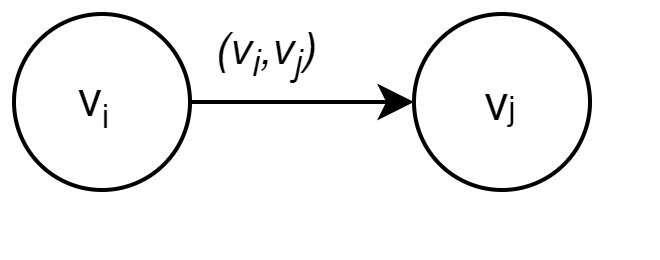
\includegraphics[scale=0.3]{figures/Multiagente/ex_grafo2.png}
    \caption{Exemplo de nós e arestas em um grafo}
    \label{fig:nos_arestas_grafos}
\end{figure}

Os graus de liberdade de entrada de um dado nó $v_i$ é definido como o número de vetores que a ponta da flecha se encontra em $v_i$. Do mesmo modo, os graus de liberdade de saída de um nó $v_i$ é dado pelo número de vetores que em $v_i$ se encontra a cauda da flecha.

Associado à cada aresta de um elemento em $E = (v_i, v_j)$ tem-se um peso $a_{ij} > 0$. O peso $a_{ij}$ representa a força de interação entre os nós $v_i$ e $v_j$. De modo que quanto maior o peso maior a influência tem o comportamento do agente $j$ sobre o agente $i$.
    %revisar esse parágrafo
Um grafo é dito bidirecional se e somente se $a_{ij} \neq 0$ e $a_{ji} \neq 0$, então tem-se que a comunicação entre agentes flui bidirecionalmente. Um grafo é dito unidirecional se $a_{ij} = a_{ji}$, para qualquer $i$ e $j$.


\section{Teoria algébrica dos grafos e consenso do controle cooperativo}

O controle cooperativo estuda a dinâmica de sistemas dinâmicos com múltiplos agentes com iterações um com o outro através de uma comunicação em grafo. 
O grafo representa as iterações e comunicações entre agentes. O objetivo do controle cooperativo é garantir a sincronia entre o comportamento e estados dos agentes, de modo que para cada agente só é disponível que as informações sejam entre o agente com os agentes vizinhos.

\subsection{Representação matricial dos grafos}
A estrutura e propriedade dos grafos podem ser estudadas examinando as propriedades de certas matrizes associadas. Dados os pesos $a{_ij}$ associados, o grafo pode ser representado pela \textbf{Matriz de Adjacência} ou conectividade $A = [a_{ij}]$, com $a_{ij}>0$ $se$ $(v_{j},v_{i}) \in E $ e $a_{ij}$ caso contrário.   
Define-se duas propriedades locais dos grafos, o graus de entrada e os graus de saída.
Os graus de entrada de um nó $v_{i}$ é definido pela equação \ref{eq:InDegree}, tal que $d_{i}$ é o somatório dos pesos $a_{ij}$ da linha $i$-th.

\begin{equation} \label{eq:InDegree}
    d_{i} = \displaystyle\sum_{j=1}^{N}a_{ij}
\end{equation}

Os graus de saída de um nó $v_{i}$ é definido pela equação \ref{eq:OutDegree}, tal que $d_{i}$ é o somatório dos pesos $a_{ij}$ da coluna $i$-th.

\begin{equation}\label{eq:OutDegree}
    d_{i}^0 = \displaystyle\sum_{j = 1}^{N}a_{ji}
\end{equation}

Define-se duas propriedades globais dos grafos, o diâmetro do grafo , dada pela maior distância entre dois nós e o volume de entrada $(in)-volume$, dado pela soma dos nós de entrada
\begin{equation}
    VolG=\displaystyle\sum_{i}d_{i}
\end{equation}

\subsection{Matriz de Grafo Laplaciana}
Uma definição importante aplicada a sistemas multiagentes é a \textbf{Matriz Laplaciana}, que auxilia o estudo das propriedades da dinâmica do grafo de multiagentes. A mesma é obtida através da operação entre duas matrize, a Matriz Diagonal e a Matriz de Adjacência.
Define-se a matriz diagonal de graus de entrada, pela equação \ref{eq:matrizDiagonal}, em que para um agente $i$, tem-se o elemento $d_{i}$ como o somatório das flechas que apontam para o dado agente.
\begin{equation}\label{eq:matrizDiagonal}
    D = diag\{d_{i}\}
\end{equation}
Por fim a matriz Laplaciana $L$ é definida como $L = D-A$, tal que $D$ é a matriz Diagonal e $A$ é a matriz de Adjacência.
\\
Um exemplo de matriz laplaciana associada ao grafo pode ser ilustrada através da figura \ref{fig:exemplo_grafo}, em que a matriz Diagonal $D$ é dada pela matriz \ref{eq:matriz_d1}. 

\begin{figure}
    \centering
    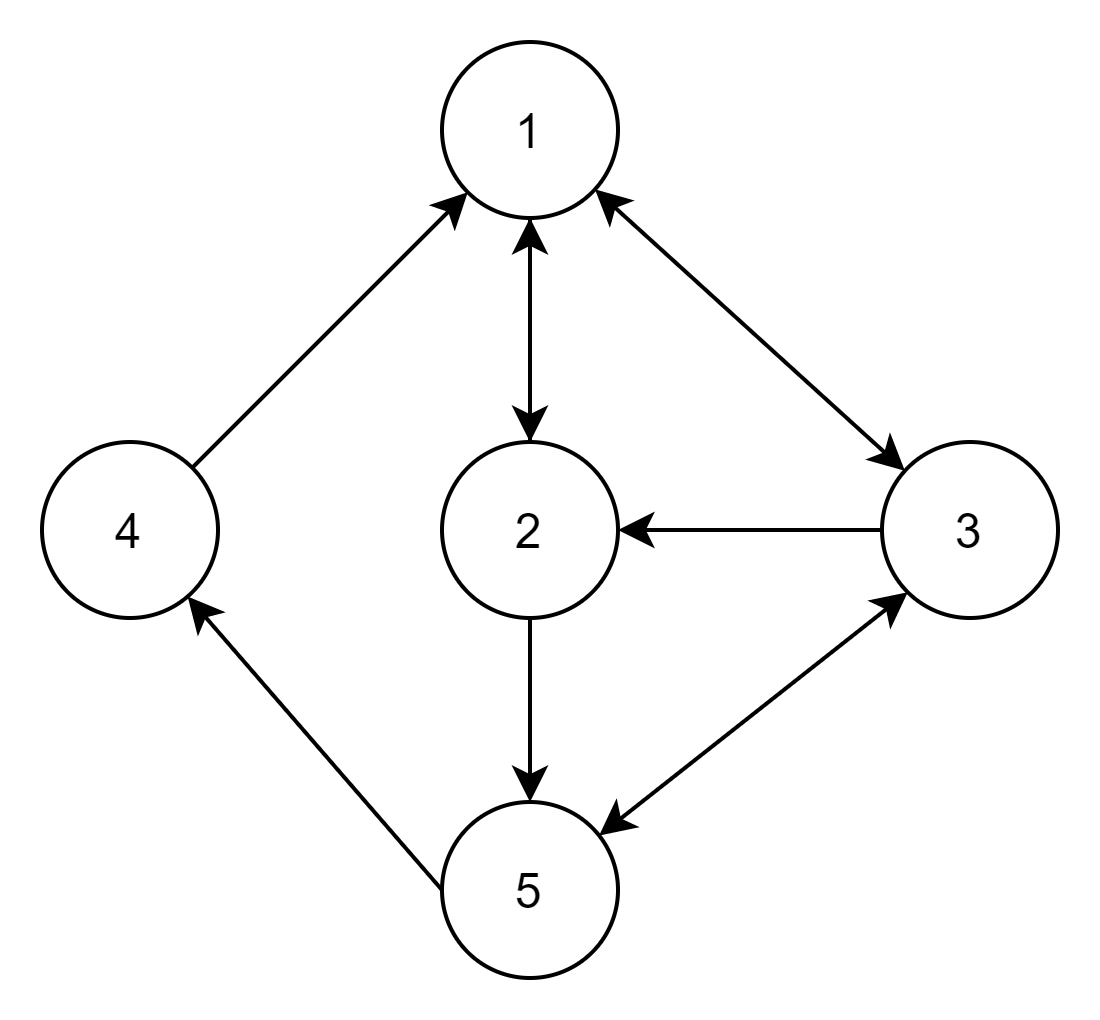
\includegraphics[scale=0.2]{figures/Multiagente/ex_grafos1.png}
    \caption{Exemplo de um grafo}
    \label{fig:exemplo_grafo}
\end{figure}

\begin{equation}\label{eq:matriz_d1}
    D = \begin{bmatrix}
         3 & 0 & 0 & 0 & 0 \\ % graus de entrada do agente 1
         0 & 2 & 0 & 0 & 0 \\ % graus de entrada do agente 2
         0 & 0 & 2 & 0 & 0 \\ % graus de entrada do agente 3
         0 & 0 & 0 & 1 & 0 \\ % graus de entrada do agente 4
         0 & 0 & 0 & 0 & 2 \\ % graus de entrada do agente 5
    \end{bmatrix}
\end{equation}

A matriz A, dada pela Matriz de Adjacência \ref{eq:matriz_A1}.
\begin{equation}\label{eq:matriz_A1}
    A = \begin{bmatrix}
         0 & 1 & 1 & 0 & 0 \\ % conectividade do agente 1  
         1 & 0 & 0 & 0 & 1 \\ % conectividade do agente 2
         1 & 1 & 0 & 0 & 1 \\ % conectividade do agente 3 
         1 & 0 & 0 & 0 & 0 \\ % conectividade do agente 4 
         0 & 0 & 1 & 1 & 0 \\ % conectividade do agente 5 
    \end{bmatrix}
\end{equation}
Por fim, a matriz Laplaciana é dada por $L = D - A$.
\begin{equation}\label{eq:matriz_L1}
    L = \begin{bmatrix}
         3 & -1 & -1 & 0 & 0 \\ 
         -1 & 2 & 0 & 0 & -1 \\ 
         -1 & -1 & 2 & 0 & -1 \\ 
         -1 & 0 & 0 & 1 & 0 \\ 
         0 & 0 & -1 & -1 & 2 \\ 
    \end{bmatrix}
    = \begin{bmatrix}
         3 & 0 & 0 & 0 & 0 \\ % graus de entrada do agente 1
         0 & 2 & 0 & 0 & 0 \\ % graus de entrada do agente 2 
         0 & 0 & 2 & 0 & 0 \\ % graus de entrada do agente 3
         0 & 0 & 0 & 1 & 0 \\ % graus de entrada do agente 4
         0 & 0 & 0 & 0 & 2 \\ % graus de entrada do agente 5
    \end{bmatrix}
    - \begin{bmatrix}
         0 & 1 & 1 & 0 & 0 \\ % conectividade do agente 1  
         1 & 0 & 0 & 0 & 1 \\ % conectividade do agente 2
         1 & 1 & 0 & 0 & 1 \\ % conectividade do agente 3 
         1 & 0 & 0 & 0 & 0 \\ % conectividade do agente 4 
         0 & 0 & 1 & 1 & 0 \\ % conectividade do agente 5 
    \end{bmatrix}
\end{equation}


\section{Consenso com Integrador único}
Para o estudo inicial de controle cooperativo, tem-se a análise de um sistema multiagente formado por agentes $i$ com dinâmica dada por um integrador escalar único, modelada pela equação \ref{eq:int_Unico}
\begin{equation}\label{eq:int_Unico}
    \dot x_{i}  = u_{i} 
\end{equation}
com $x_{i}, u_{i} \in R $ . Isso corresponde que cada nó do grafo $G$, possui um agente com memória.

\subsubsection{Protocolo de controle distribuído para o consenso}
Para cada agente $i$, considere o protocolo de controle local dado pela equação \ref{eq:protocolo_controle_local}
\begin{equation}\label{eq:protocolo_controle_local}
    u_{i} = \sum\limits_{j \in N_{i}} a_{ij} (x_{j} - x_{i})
\end{equation}
com $a_{ij}$ sendo o peso de interação entre os estados dos agentes.Essa equação é conhecida como protocolo de votação local, em que o estado de cada agente depende tão somente do estado do agente vizinho, e a entrada de controle depende da da diferença dos estados em relação aos agentes vizinhos. De modo que percebe-se que se todos os estados forem os mesmo a entrada de controle tende a zero $\dot x_{i} = u_{i} = 0$.

Para a dinâmica de integrador único, é desejável que a equação \ref{eq:int_Unico}, resolva o problema de consenso, da dinâmica de malha fechada dada pela equação \ref{eq:consenso_Int_Unico}
\begin{equation}\label{eq:consenso_Int_Unico}
    \dot x_{i} = \sum\limits_{j \in N_{i}} a_{ij} (x_{j} - x_{i})
\end{equation}

Reorganizando a equação \ref{eq:consenso_Int_Unico}, tem-se que a equação. \ref{eq:consenso_Int_Unico_Expandido}
\begin{equation}\label{eq:consenso_Int_Unico_Expandido}
    \dot x_{i} = -x_{i}\sum\limits_{j \in N_{i}} a_{ij} + 
    \sum\limits_{j \in N_{i}} a_{ij}x_{j} = -d_{i}x_{i} + 
   \left[
   \begin{array}{ccc}
   a_{i1}&\cdots&a_{iN} 
    \end{array}
    \right] 
   \left[
   \begin{array}{ccc}
        x_{1} \\
        \vdots \\
        x_{N}
    \end{array}
    \right]
\end{equation}
tal que $d_{i}$ são os graus de liberdade, $x = [x_{1} \cdots x_{N}]$ $\in R^N$ o vetor de estados. Define-se a matriz $D$ como matriz diagonal formada por $D = diag \{d_{i}\}$, organiza-se a 
dinâmica global, através da matriz dada pela equação Laplaciana.
\begin{equation}\label{eq:construcao_laplaciana}
    \begin{aligned}
        \dot x = -Dx +Ax = -(D-A)x \\
        \dot x = u = -Lx 
    \end{aligned}
\end{equation}
Através da equação \ref{eq:construcao_laplaciana}, e da matriz laplaciana de grafo tem-se que a dinâmica de malha fechada pode ser analisada através da matriz laplaciana dada.
Para a dinâmica de integrador único tem-se que se e somente se o grafo possui a topologia de spanning tree, então todos os estados dos nós vão a um valor de consenso dado por $x_{i} = x_{j} = c$. O valor de consenso é dado pela equação \ref{eq:valor_de_consenso}.
\begin{equation}\label{eq:valor_de_consenso}
    \begin{aligned}
        c = \sum\limits_{i = 1}^{N} p_{i}x_{i}(0)
    \end{aligned}
\end{equation}
tal que $w_{1} = [p_{1} \cdots p_{N}]^{T}$, é o vetor normalizado pela esquerda da matriz laplaciana $L$, para $  \lambda_{1} = 0$. De modo que a constante de tempo é dada por \ref{eq:const_tempo} e $\lambda_{2}$ sendo o segundo autovalor da matriz L.
\begin{equation}\label{eq:const_tempo}
   \tau = 1 / \lambda_{2}
\end{equation}


\subsection{Consenso com líder}
Um "(directed) tree" é um um grafo onde todo nó exceto um é chamado de líder, e possui grau de entrada unitário. De modo que todos os outros nós possuem um consenso liderado pelas condições iniciais do líder.
O valor de consenso é dado pela equação \ref{eq:valor_de_consenso}, de modo que $p_{i}$ é o $i-{th}$ componente para o autovetor pela esquerda de $w_{i}$ para $\lambda_{1} = 0$, tal consenso é na verdade a média ponderada das condições iniciais das raízes dos nós ou do líder em um grafo. 
%% Adicionar simulação parecida com a simulação da pág 42 do livro, sobre consenso com líder.
\\
\\
\subsection{Consenso para nós com estados como vetores}
Nas condições de integrador úninco e integrado duplo apresentadas anteriormente os estados são tidos como escalares, para os exemplos em que os estados são vetores tais como $x_{i}, u_{i} \in R^{N}$ tem-se que os vetores globais de estados e controle são respectivamente $x = [x_{1}^{T} \cdots x_{N}^{T}]^{T} \in R^{nN} , 
u = [u_{1}^{T}  \cdots u_{N}^{T}]^{T} \in R^{nN} $ e os elementos dados pelos pesos de consenso $a_{ij}$ e a diagonal $d_{i}$ são multiplicados pela matriz identidade $I_{n}$, de modo que a dinâmica global do sistema é dada pela equação \ref{eq:consenso_vetorial}

\begin{equation}\label{eq:consenso_vetorial}
 \begin{aligned}
    u = -(L \otimes I_{N})x \\
    \dot x = -(L \otimes I_{N}) x
    \end{aligned}
\end{equation}
dado que $\otimes$ é definido como produto de kronecker.

\subsection{Movimento invariante para consenso de primeira ordem}
Para o protocolo de primeira ordem local dado por \ref{eq:construcao_laplaciana} foi garantido que para a topologia de $spannig tree$ o consenso é alcançado. 


